\section{Функционал шаардлагууд}
\begin{table}[h!]
	\centering
	\begin{tabular}{ |p{2cm}|p{13cm}| }
      \hline
      ФШ 100 & Систем нь лиценз идэвхжүүлэх үйл явцын үнэн зөв, бүрэн бүтэн байдлыг хангахын тулд блокчейн технологийг ашиглана.
      \\ \hline
      ФШ 200 & Хэрэглэгчид  лицензийнхээ талаарх дэлгэрэнгүй мэдээллийг харах боломжтой байх ёстой.
      \\ \hline
      ФШ 300 & Хэрэглэгчдэд лицензээ найдвартай шилжүүлэх, хуваалцах функцийг хэрэгжүүлэх.
      \\ \hline
      ФШ 400 & Шилжүүлэх үйл явцыг автоматжуулах, баталгаажуулахын тулд блокчейны ухаалаг гэрээг ашиглана.
      \\ \hline
      ФШ 500 & Хэрэглэгчид лицензийн хугацаа дуусахаас өмнө эсвэл дуусахад сунгах боломжтой байх ёстой.
      \\ \hline
      ФШ 600 & Систем нь хэрэглэгчдэд лицензийнхээ жинхэнэ эсэхийг шалгах, баталгаажуулах боломжтой байх.
      \\ \hline
	\end{tabular}
   \caption{Функциональ шаардлага}
\end{table}

\newpage
\section{Функционал бус шаардлагууд}
\begin{table}[h!]
	\centering
	\begin{tabular}{ |p{2cm}|p{13cm}| }
		\hline
		ФБШ 100 & Блокчейн технологи нь өгөгдлийн бүрэн бүтэн байдлыг хангаж, лицензийн мэдээллийг зөвшөөрөлгүй өөрчлөхөөс сэргийлнэ.
      \\ \hline
		ФБШ 200 & Систем нь гүйцэтгэлийн бууралтгүйгээр олон тооны хэрэглэгчид болон лицензүүдийг зохицуулах чадвартай байх ёстой.
      \\ \hline
		ФБШ 300 & Ухаалаг гэрээ нь модульчлагдсан байх ёстой бөгөөд шинэчлэгдэхэд хялбар байх ёстой.
      \\ \hline
		ФБШ 400 & Систем нь хүлээн зөвшөөрөгдсөн тодорхой хугацааны дотор гарын үсэг үүсгэх, баталгаажуулах хүсэлтийг хурдан боловсруулах чадвартай байх ёстой.
      \\ \hline
		ФБШ 500 & Систем нь янз бүрийн техникийн чадвартай хэрэглэгчдэд үүнийг үр дүнтэй ашиглах боломжийг олгодог хэрэглэгчдэд ээлтэй интерфэйстэй байх ёстой.
      \\ \hline
		ФБШ 600 & Систем нь лиценз олгох, дижитал гүйлгээ, блокчэйн технологитой холбоотой аливаа зохицуулалтын шаардлагад нийцэж байх.
      \\  \hline
      ФБШ 700 & Энэ систем нь гамшгийн үед өгөгдөл алдагдахгүй байхын тулд найдвартай нөөцлөх, сэргээх механизмтай байх ёстой.
      \\ \hline
	\end{tabular}
   \caption{Функциональ бус шаардлага}
\end{table}

% \section{Use-case диаграм}
% \begin{figure}[h]
% 	\centering
% 	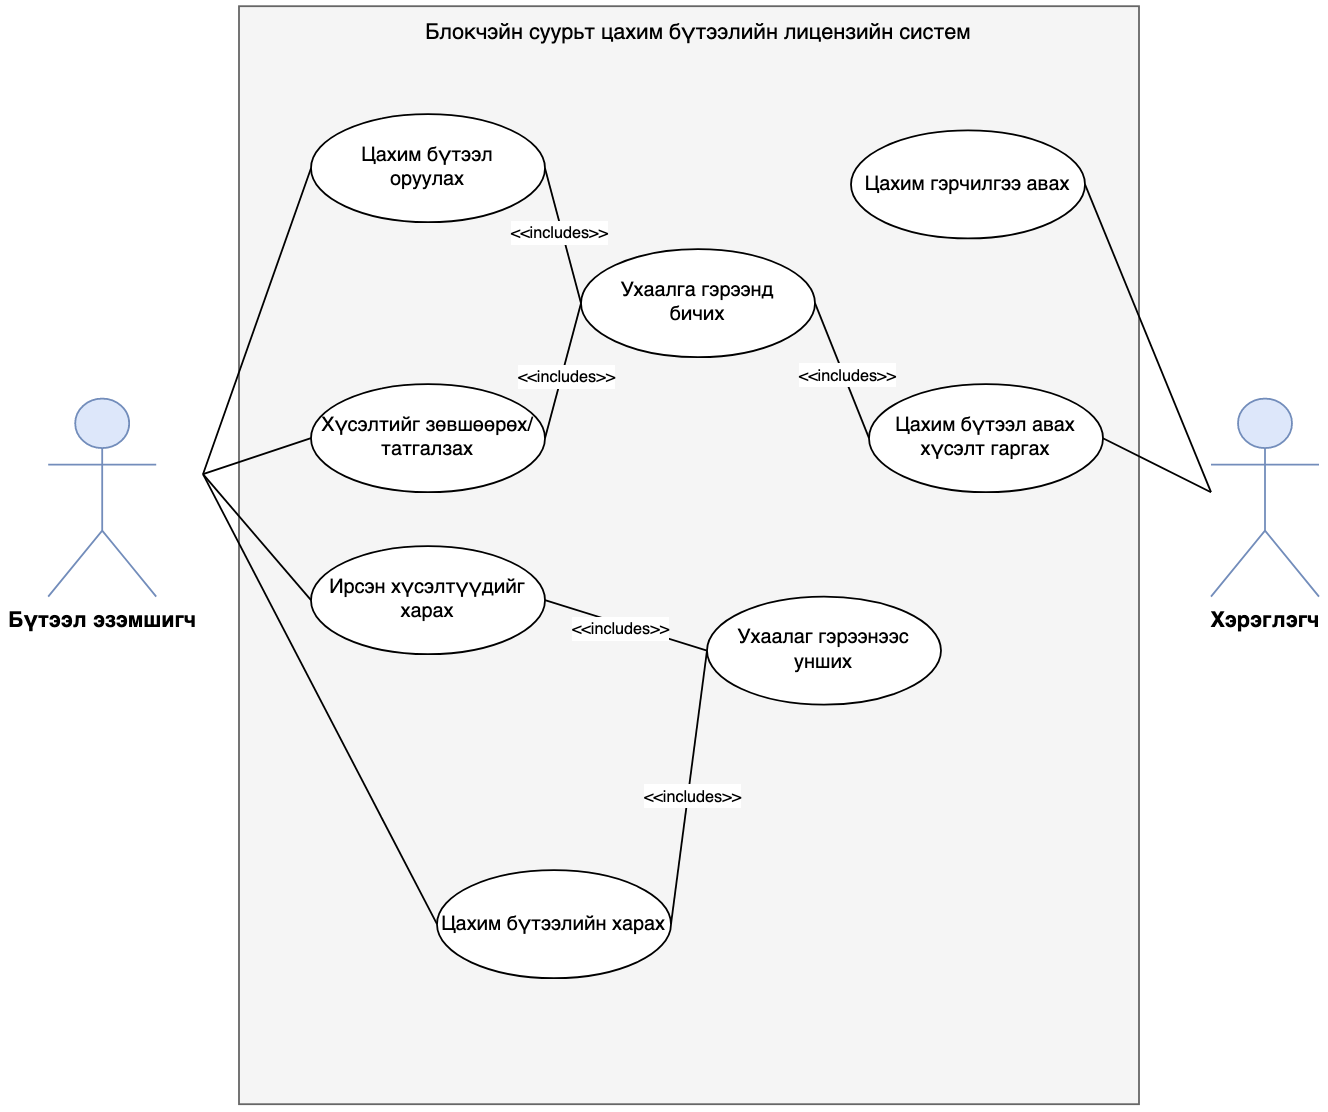
\includegraphics[scale=0.3]{src/images/usecase.png}
% 	\caption{Use-case диаграм}
% \end{figure}
